\section{Rethinking storage for Docker registry}
\label{sec:file_adressable}
%
%\NZ{The main goal of this section is to provide some hints for designer to implement a fast dedup system.
%	We do not give any design in the workshop paper. We will keep performance analysis and simulation part, 
%	just give some basic latencies for each involved operations for designer to think about how to improve their design and what will be the bottleneck.
%	}
%
In this section we propose a file-level content addressable storage model (FLCAS)
based on file-level deduplication
for Docker as an alternative to layer-level content addressable storage.
%
% and save space while maintaing good
%FLCAS, can significantly reduce the redundant files in docker registry and save
%a large volume of storage space.
%
While FLCAS can significantly reduce the number of redundant files in the Docker
registry, it comes with several challenges, 
including file-level deduplication overhead and its impact on push or pull latencies.
For example, after layers are pushed in registry, FLCAS decompresses the layer archival files,
calculates the file content digests, searches whether the identical files are stored or not. 
If not, FLCAS stores these unique files.
%
These above operations are either CPU intensive or I/O intensive, which would impact 
the foreground push/pull requests.
%
Upon a pull request, FLCAS first restores the requested 
layer archival files by fetching all its containing files and compressing them.
%
The overhead of restoring a layer would become a bottleneck of a pull request.
%
How to manage layer-to-file mapping to provide fast searching \& indexing performance 
is also a challenging to FLCAS.
%file-level deduplication not only includes calculation of file content digest, 
%searching for identical files, and storing unique files, 
%but also includes decompression of layer archival files and and restoring layer archival files.
%decompression of layer archival files,
%calculation of file content digest, 
%searching for identical files, 
%storing unique files,
%and restoring layer archival files.
%
\LR{The challenges are not clear at this point. We need to first briefly describe the
overall approach, i.e. layer is pushed, archive is decompressed, file digests are
calculated, etc., and then say, what exactly is challenging/problematic about this
approach.}\NZ{addressed}
\LR{The challenges should also be connected back to their effect, i.e. they will
affect push and pull latencies.}\NZ{addressed}
\LR{We should also add the layer reconstruction as another challenge.}
\LR{Another challenge could be dealing with files that have same data but different
metadata.}\NZ{addressed}
%

To analyze the impact of file-level deduplication, we simulate a simple FLCAS on
0.9 million layers and measure the performance for each step of the approach.
%
Based on this analysis, we identify which operation is likely to become the bottleneck
and as a result increases \texttt{push} and \texttt{pull} layer request latencies.
\LR{Make sure commands are consistent throughout the paper. Usually, commands
are displayed in a \texttt{texttt} block.} \NZ{addressed}
%we explain how FLCAS supports \emph{push layer} and \emph{pull layer}
%requests.
%
We then provide different suggestions on how the Docker registry can mitigate
the deduplication overhead.
% and efficiently server push/pull requests.
%

\subsection{Performance analysis}
%
\begin{figure}
	\centering
	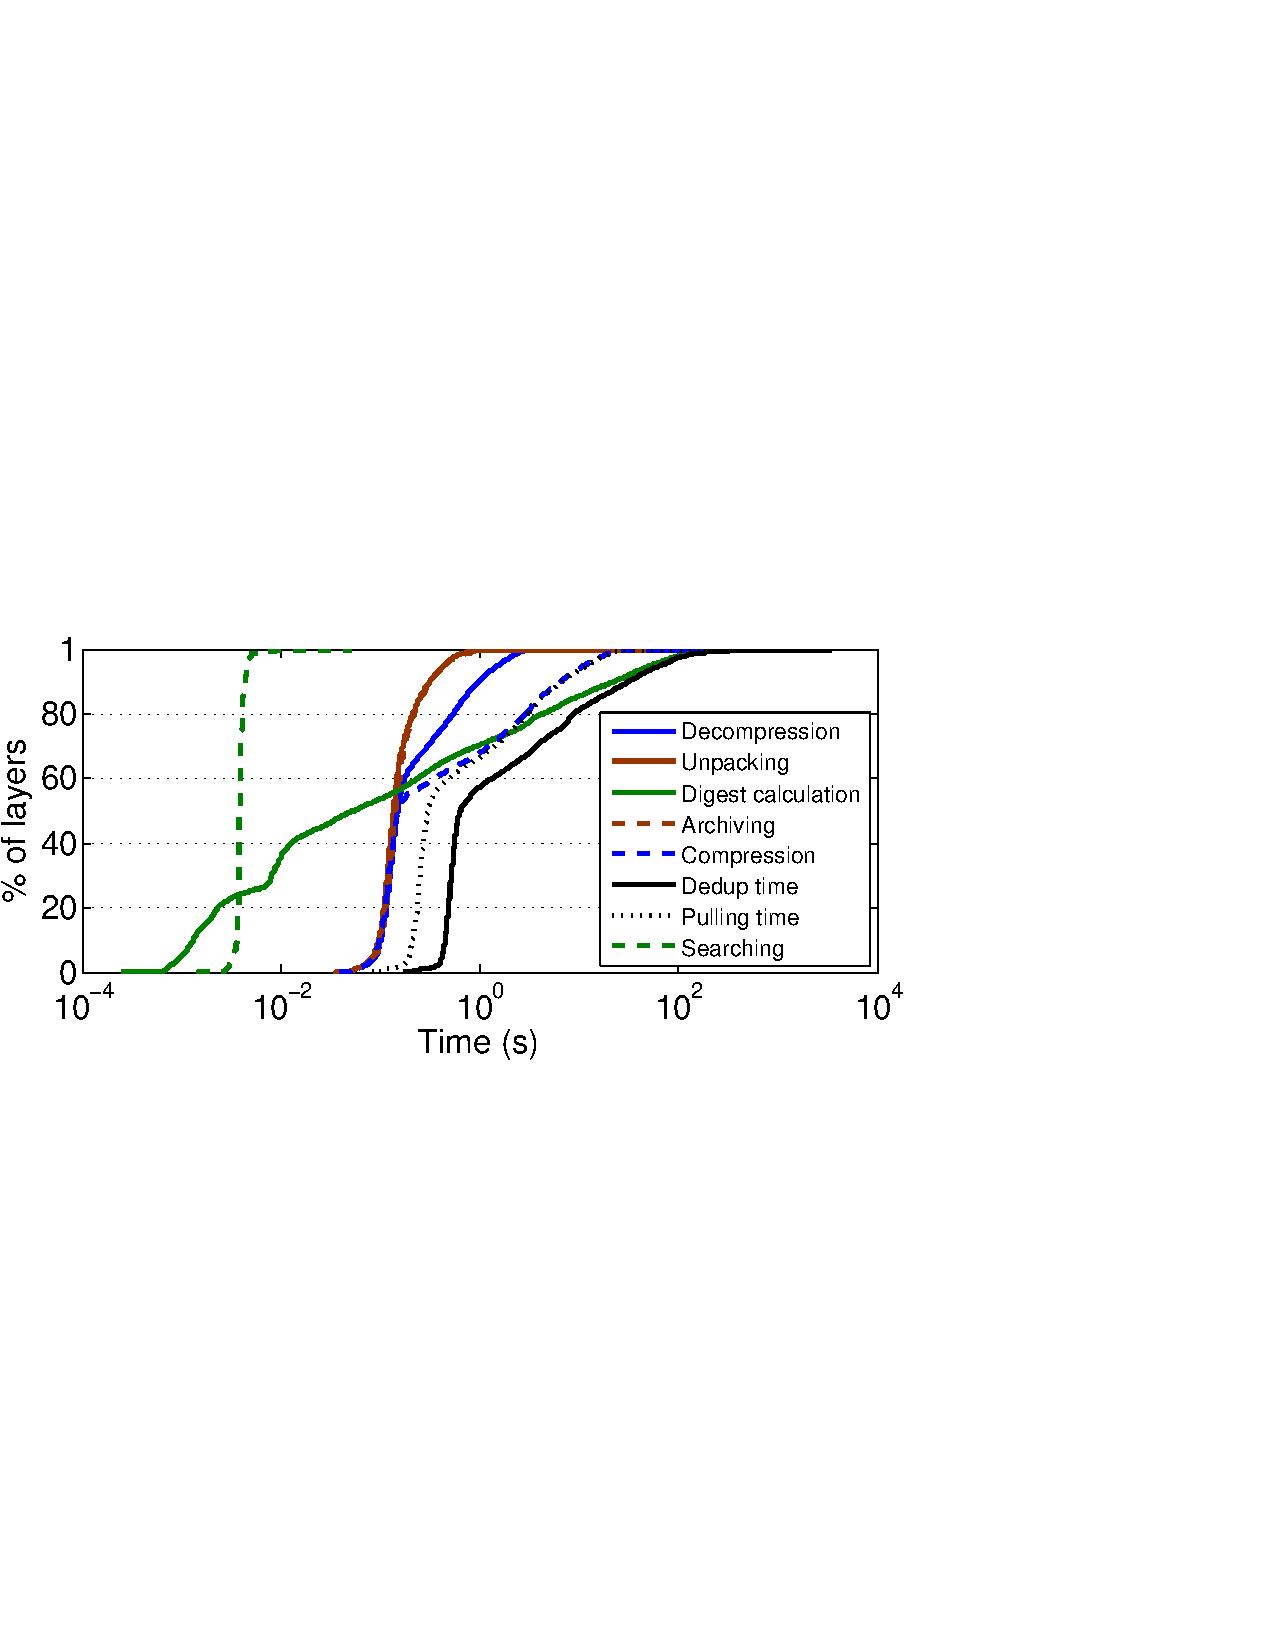
\includegraphics[width=0.4\textwidth]{graphs/res-time.pdf}
	\caption{Off-line file-level deduplication run time.
	\LR{What is ``off-line''? Hasn't been introduced.}\NZ{addressed}}
	\label{fig:dedup-res}
\end{figure}


%\paragraph{Simulation} 
%
% since dedup process only starts periodically when the
%workload is lower and only cold layers are evolved in dedup process (discussed
%in Section~\ref{subsec:FLCAS}).
%
%\lrcomment{By latency, do you mean the time it takes to perform the dedup? I
%wouldn't call that latency but rather run time or completion time.}
%
%\lrcomment{What exactly was the setup? Where those 60 requests submitted while
%the dedup was running and where they submitted only once or repeatedly?}

\LR{I think the flow in this subsection can be improved. Instead of the ``file-level deduplication
run time'' paragraph, I would introduce Fig~\ref{fig:dedup-res} at the end of the first paragraph,
right before ``Push layer latency'' and maybe explain the overal run time there. In the push and pull
layer latency we can then focus on just the parts of the graph that are related to push and pull.
This would be a more top-down presentation (which I feel often works better in papers).}
%\NZ{addressed}

\LR{I'm still not sure if we should use simulation or emulation?}
To study the overhead of file-level deduplication, we setup a
one-node Docker registry with 64~GB RAM and 32 Cores.  
%
We wrote around 600 lines of Python code to perform \emph{off-line} file-level deduplication
operations on the layer dataset.
%

\LR{We can remove the following steps once we explained them better
in 4.0}\NZ{addressed}
% 
%File-level deduplication mainly
%consists of the following steps: 
%layer decompression, 
%file content digest calculation,
%searching \& indexing,
%and storing unique files.
%The unique files are stored in a \textit{file pool}.

Our simulation follows the steps of FLACS as explained above:
First, a layer from the layer dataset is read and copied
to a RAM disk. The layer is then decompressed and 
the digests for each individual file are computed by using MD5 hash function~\cite{MD5}.
\LR{How is the digest computed?}\NZ{addressed}
%
\LR{\emph{emph} should be used instead of \textit{textit} to
emphasize certain words/parts in the text.}\NZ{addressed}
If the file is not \emph{stored},
we record the \emph{file content address}, which is a
file digest linked to the files' location.
%And we append a \textit{layer-to-file} 
%mapping record to a mapping table. 
%
\LR{This part is confusing. What does ``layer digest to its containing file content
digest mapping record'' mean? Why is it for each file in a layer and all layers?}
\NZ{addressed}
To map a layer to it's containing files, we create a \emph{layer-to-file} record
%For each file in a layer, 
%a layer digest
%to its containing file content digest mapping record is also created 
and save it
to a \emph{layer-to-file table}.
%
The \emph{layer-to-file table} also
records the file path within each layer associated with each file.
%
Note that we do not consider the latency of storing unique files in our simulation.
%
%Only unique files are maintained in RAM
%disk while the redundant copies are removed.
%
We run FLCAS for 0.9 Million layers in total and process 60 layers concurrently. 
%
Overall, it took 3.5 days to finish.
%
%
%The overall runtime is about 3.5 days.

\LR{What was the overall runtime for processing 0.9 million layers?}\NZ{addressed}
%
%\alicomment{How are we saving the location
%of each file in the layer? It is not clear from the following sentences.}
%\NZ{addressed}
%
%To improve searching performance, the
%mapping table is stored in Hive database~\cite{xxx}. 
%
%\lrcomment{Why are we using Hive for this? It seems overkill to me, especially
%for such small data. Even at scale, a KeyValue store would probably provide
%better performance than clunky MapReduce-based DB.}
%

\paragraph{Push layer latency}

FLCAS does not affect the latency of \emph{push layer} requests
because before performing deduplication, the registry reliably stores
a copy of the layer as is and then sends a response message to the user.
%
Hence, no addition delay will be added to the pushing time. 
%
\paragraph{Pull layer latency} 

For a \emph{pull layer} requests, the registry will first fetch 
all its containing files by consulting the \emph{layer-to-file table}, 
restore the layer archive file by compressing these files, and
then send the compressed layer archive file to the clients.

Figure~\ref{fig:dedup-res} shows a breakdown of the \emph{pull layer}
latency.
%
Note that the \emph{pull layer} latency is the sum of archiving time,
compression time, and searching time and does not include network transfer
time. 
%
\LR{Always add a protected space or a \textbackslash, between a number and its unit.}
\NZ{addressed}
We can see that around 55\% of the layers have a similar compression and archiving
time ranging from from 0.04\,s to 0.15\,s and both operations contribute equally
to pulling latency.
%60\% of compression and archiving time are less than 0.15 s.
%
%While compression has the highest run time 80\% of compression time is less than 2.82~s. 
%
After that, the times diverge and compression times increase faster with an
80\textsuperscript{ts} percentile of 2.82\,s. Hence, compression time makes
up the major portion of the pull latency and becomes a bottleneck.
This is because that the layer size is big\LR{put reason here}
\NZ{I think the layer size is the major reason}.
%
%We see that archiving time and compression contributes equally to pulling
%latency when their run time are lower than 0.15 s while compression time almost
%equals to pulling latency when the compression time is greater than 0.15 s. 
%
To reduce latency, we suggest that fast compression methods should be applied reduce
compression time. As deduplication provides significant storage savings, faster compression
methods with a lower compression ratio are hence feasible.

%\alicomment{Separately mention pull layer requests}
%

\paragraph{File-level deduplication run time}

%and pulling requests for  
%
\LR{This should go under ``Push layer latency''}\NZ{dedup time won't affect the push latency. 
	So we cannot discuss the following latencies in push layer paragraph.}
Figure~\ref{fig:dedup-res} shows the breakdown of run time for each
involved operation: decompression time, unpacking time, file content digest
calculation time, and searching time.
First, among all the operations, we see that searching time is the
smallest. 
%
80\% of searching time is less than 0.004\,s. 
%
The mapping table
maintains 0.98 million layer-to-file digest mapping records. 
%
\LR{Remove the following sentence? 1.7 million records is actually quite
small so even a single-node DB with one index is enough.}\NZ{addressed}
%
%Consider that more
%than 1.7 million layers are stored in Docker hub and the number is still
%increasing, it's better to choose a fast distributed database to provide high
%searching performance and scalability.
%
%\lrcomment{How does our DB schema look and what are the search queries?}

\LR{This should go under ``Push layer latency''}
Second, we see that digest calculation time spreads over a large range started
from 0.000005 s to 124.7\,s. 
%
This is because digest calculation time mainly
depends on the layer size., \ie the less and smaller files a layer
contains, the faster it is to compute all digests for the layer.
%
%Typically, smaller layers contain a smaller number
%of smaller files, which takes much less time to calculate their digests.
%
%While if the layer is bigger, the digest calculation overhead will be higher. 
%
80\% of digest calculation time is less than 4.21\,s. 
%
Thus, we suggest that multiple-threading is needed to calculate the files'
digests simultaneously; 
%
Fast CPUs as well as more powerful computing nodes are
required to speed up digest calculation.

\LR{This should go under ``Push layer latency''}
\LR{This is pretty much equal to Archiving and Compression times. Does
that mean in those cases, we're I/O bound?}
\NZ{no, we use RAM disk for storing all layers both in decompressed/compressed format.
decompresson/compression time depends on layer size, I think.}
Third, the run time for decompression and unpacking have the same distribution
during the lowest response time range started from 0.04\,s to 0.15\,s. 
%
Around 60\% of decompression and unpacking time are less than 0.15\,s. 
%
However, decompression has the highest time than that of unpacking. 
%
80\% of decompression is less than 0.55 s while 80\% of packing time is less than 0.21\,s. 

\LR{This should go at the end of the first part of Section 4.1 and before ``Push layer
	latency''}
Figure~\ref{fig:dedup-res} shows the total time distribution for
file-level deduplication which is the sum of run time for decompression, unpacking,
digest calculation, and searching. 
%
We see that 80\% of file-level dedup time is
less than 9.09\,s per layer.
%
%\lrcomment{Is that per layer or per file or per image?}
%
We also measured the throughput of 60 processes. 
%
Our one-node file-level
deduplication prototype can process about 3\,layers/s. 
%
We suggest to use more
high powerful machines to improve throughput.
 
%
\subsection{Improving the performance of FLCAS}

Based on our simulation results, we propose two optimizations
to speed up pull requests when file-level deduplication is used
in a registry.

\paragraph{Deduplicating when workload is light}

As shown above, file-level deduplication comes with some performance overhead.
%
However, the registries often experience fluctuationg workloads with
peaks and troughs~\cite{dockerworkload}.
%
%Also, 80\% of the time, registry serves only 100 or less requests.
%
\LR{This is confusing. From our previous description, it sounded like we're
performing deduplication every time a layer gets pushed. What exactly does it mean
to ``trigger it for cold layers'' and why do we need to do that? Explain better.}
\NZ{we did a off-line simulation. I mentioned in the first paragraph in performance analysis}
%
So file-level dedupilication can be triggered for removing the redundant files 
only when the workload is low and storage utilization is high.
%
To further improve the performance of FLCAS, we also suggest to use main memory
for temporarily storing and processing \textit{small} layers.
%
According to our findings (see~\S\ref{sec:dedup_ratio}), the majority of layers~(87.3\%)
are smaller than 50\,MB and hence can be stored and processed in RAM to speed up
deduplication. 

\begin{figure}
	\centering
	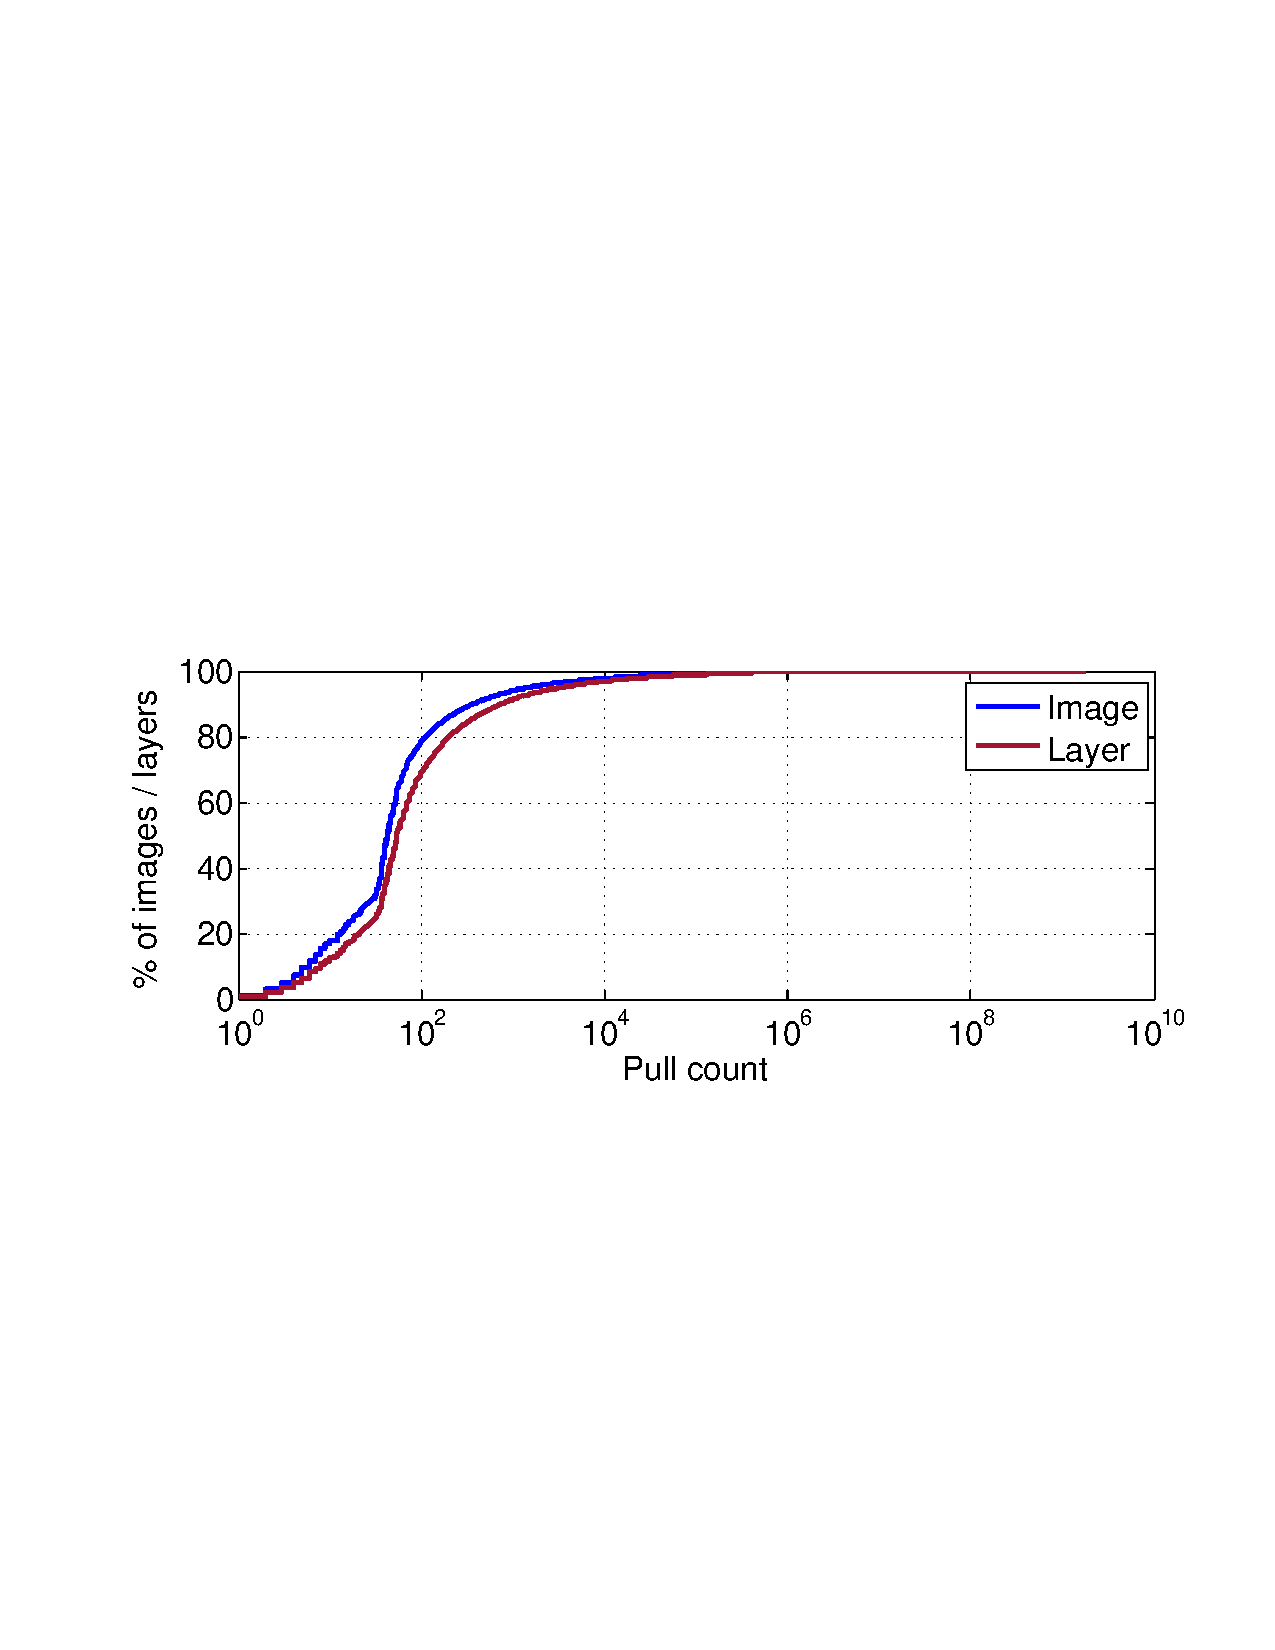
\includegraphics[width=0.4\textwidth]{graphs/pull-cnt.pdf}
	\caption{CDF of layer \& image pull count.
	}
	\label{fig:pull-cnt}
\end{figure}

\paragraph{Caching hot layers}

To further reduce overhead, we propose to cache the hot/recently requested layers as
gzip compressed tar files.
%
We observe that only a small proportion of images
and layers are frequently requested and majority of images and layers are
\textit{cold}.
%
Figure~\ref{fig:pull-cnt} shows the total
number of pulls from the time an image/layer has been stored in Docker Hub until
May 30, 2017.
%
We see that only 20\% and 10\% of images are pulled more than 100 and
360 times respectively.
%
Similarly, only 20\% and 10\% of layers are pulled
more than 217 and 660 times.
%
Note that we calculate the layer pull count shown in
Figure~\ref{fig:pull-cnt} by aggregating the pull count of
all images, which refer to this layer.
%
%Note that the image pull counts are crawled
%from Docker Hub website.
%
Actual layer pull counts should be less because pulling an image does not
necessarily pull all its containing layers if some layer have been previously
downloaded and are already available locally.
%

%
%\lrcomment{How does this compare to pulling without dedup? What's the overhead
%added?}


%
%\vcomment{What are the units for  $\sigma_{wl}$ and  $\sigma_{su}$?}
%
%\lrcomment{Do you mean it only runs through low workload periods? How are we
%predicting those or are we relying on some workload patterns? We should make
%that clear.}

%high while start file-level dedup \paragraph{FLCAS model}
%Figure~\ref{fig:file-dedup-model} shows an example of FLCAS.
%
%\vcomment{An example?..}
%
%\lrcomment{This explanation should come before the caching and light workloads
%paragraphs.}
%

%\paragraph{Caching hot layers to improve performance}
%\label{subsec:FLCAS}
%
%\begin{figure}
%	\centering
%	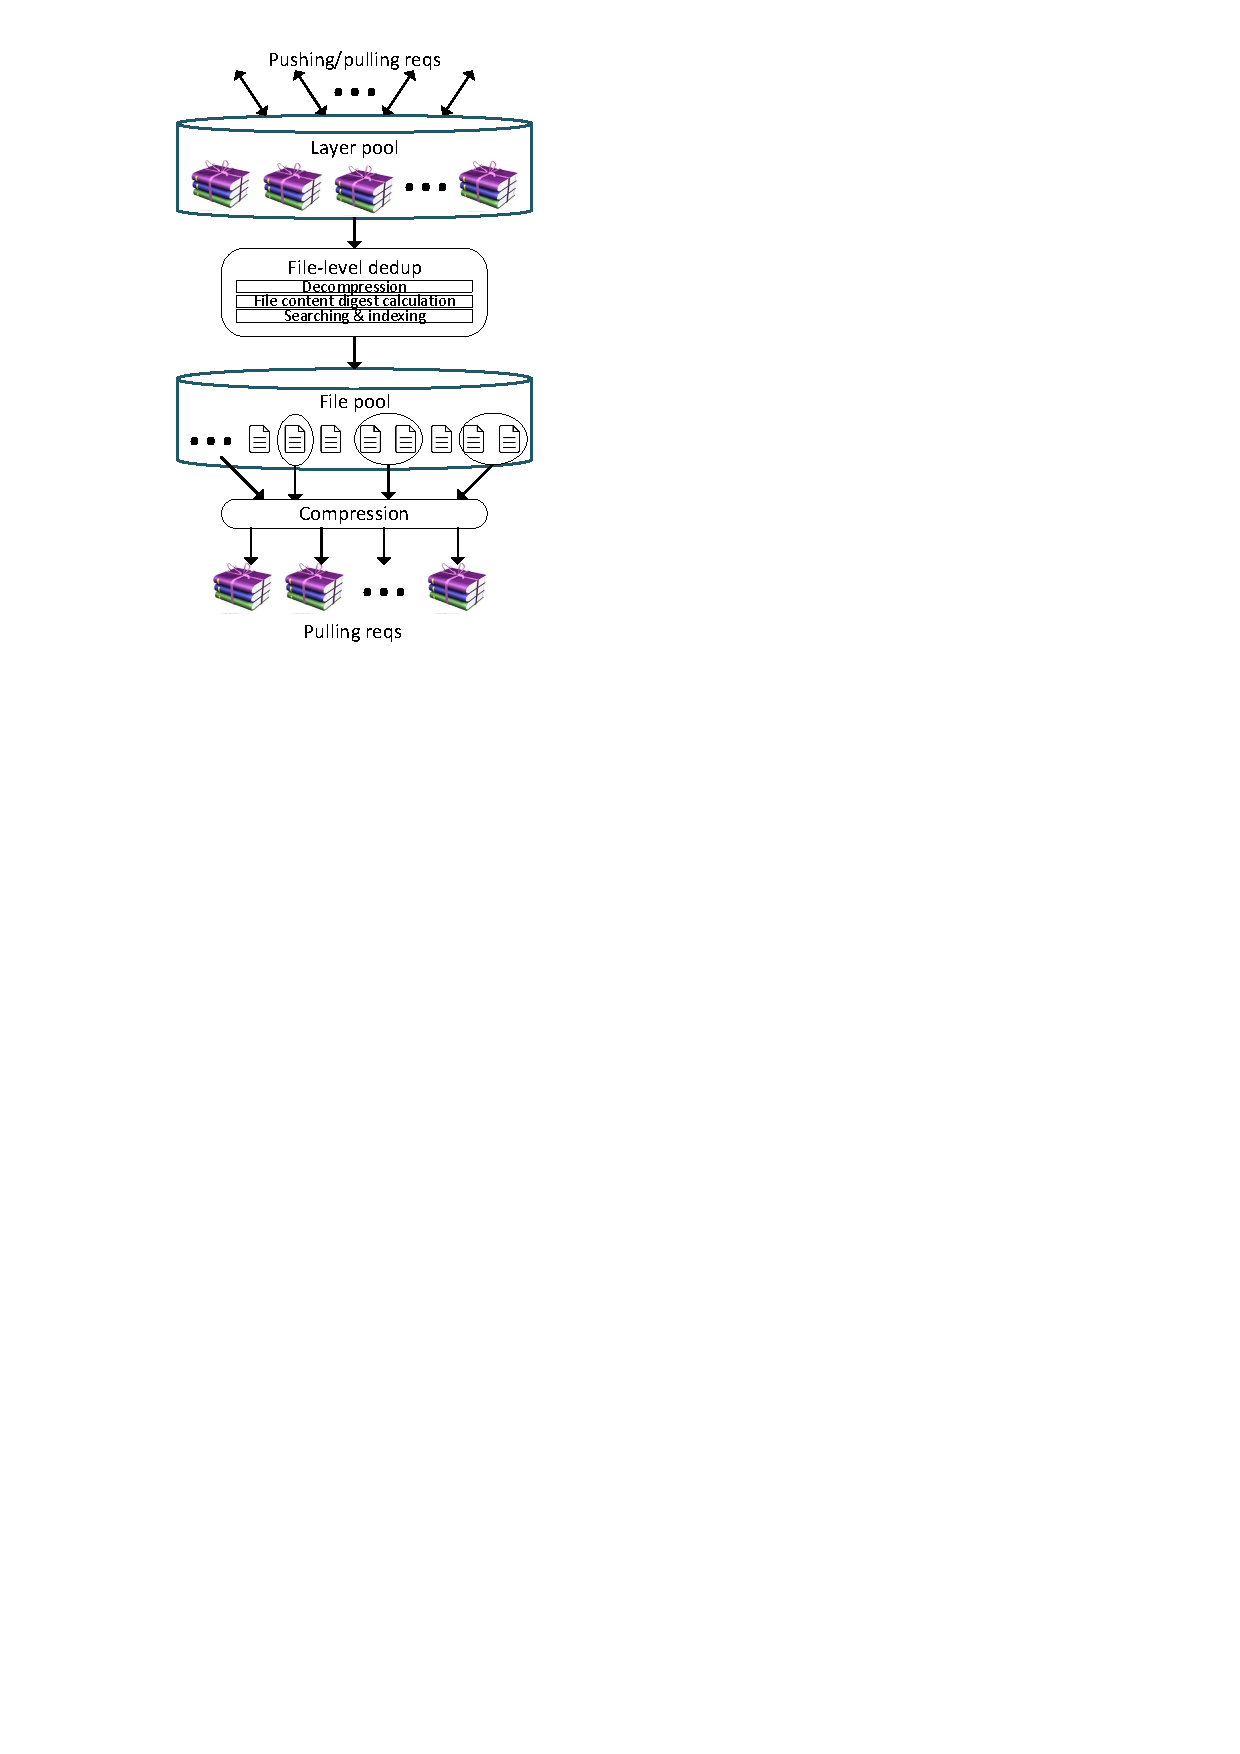
\includegraphics[width=0.3\textwidth]{graphs/graph_compression_layers.pdf}
%	\caption{File-level content addressable model.
%	\vcomment{1) Do not see ``cache'' word on the figure. 2) Font is too small in the middle section. 3) We need to describe how we depict layers vs. files. 4) There are pull requests both from the top and the bottom . I think we should just remove the part below the File pool.}
%	}
%	\label{fig:file-dedup-model}
%\end{figure}

%
%\vcomment{Who is ``it''?}\nancomment{addressed}
%
%
%\vcomment{Who are ``they''? Avoid using ``it'' and ``they''. Use actual nouns instead.}
%
 %a digest generated by a cryptographic hash function (such as ) 
%
%\vcomment{Let's use ``deduplication'' instead of ``dedup'' everywhere (because
%the letter one is informal)}

%\subsection{Trade-off discussion}

%

%\vcomment{I think there are two reasons for the cache 1) reduce push latency
%and 2) reduce pull latency. The text above talks only about reducing pull
%latencies.  We also need to talk about pushes.  Furthermore, the current
%discussion of pull counts does not really justify read (pull) cache.  For the
%read (pull) cache to be efficient there should be many pulls that access the
%same layers. E.g., that XXX\% of pulls go to the few YYY popular layers.
%Can we say that?}
%%
%\vcomment{somewhere we will need to talk about eviction policy, how to
%size the caching layer, and, finally, what happens if the cache is full.}
% 

%\subsection{Using RAM to load \&. process layers}
%
%To improve performance, we use RAM to temporarily store \textit{small} layers
%and directly process them in RAM.  Specially, we first load small layers in a
%RAM disk and perform decompression, unpacking, file content digest calculation
%in RAM, and remove them from RAM after completion.   According to our findings
%that majority (87.3\%) of layers that are less than 50M as shown in
%Figure~\ref{fig:image-layer-size}. So majority of layers can be stored and
%processed in RAM to speed up file-level dedup. 
%%layers that are less than 50M are stored and processed in RAM while the rest
%%layers are stored and processed in SSDs.
%%
%\lrcomment{This should still be part of 7.1 as it explains the strategy and not
%the prototype/simulations.}
%%
%\lrcomment{How are small layers defined? Where is the threshold?}
%
%majority (xxx) of layers'dedup times are less than xxx.
%during peak workload, which means that we start file-level dedup whenever it receives a layer. 
%To simulate the high intensive workload, we first sent a sequential of layer pushing requests to registry and stored, then we measure the file-level dedup  
%, archiving time, and compression time.
%Second, compare the latency for each operation, we see that xxxx
%\paragraph{Latency breakdown}
%We calculated the latency for each operation for all layers as shown as Table~\ref{tbl:latency_breakdown}.
%Figure~\ref{xxx} shows the compression time across 

%\begin{figure}[!t]
%	\centering
%	\subfigure[CDF of repositories by pull count]{\label{fig_pull_cnt_total}
%		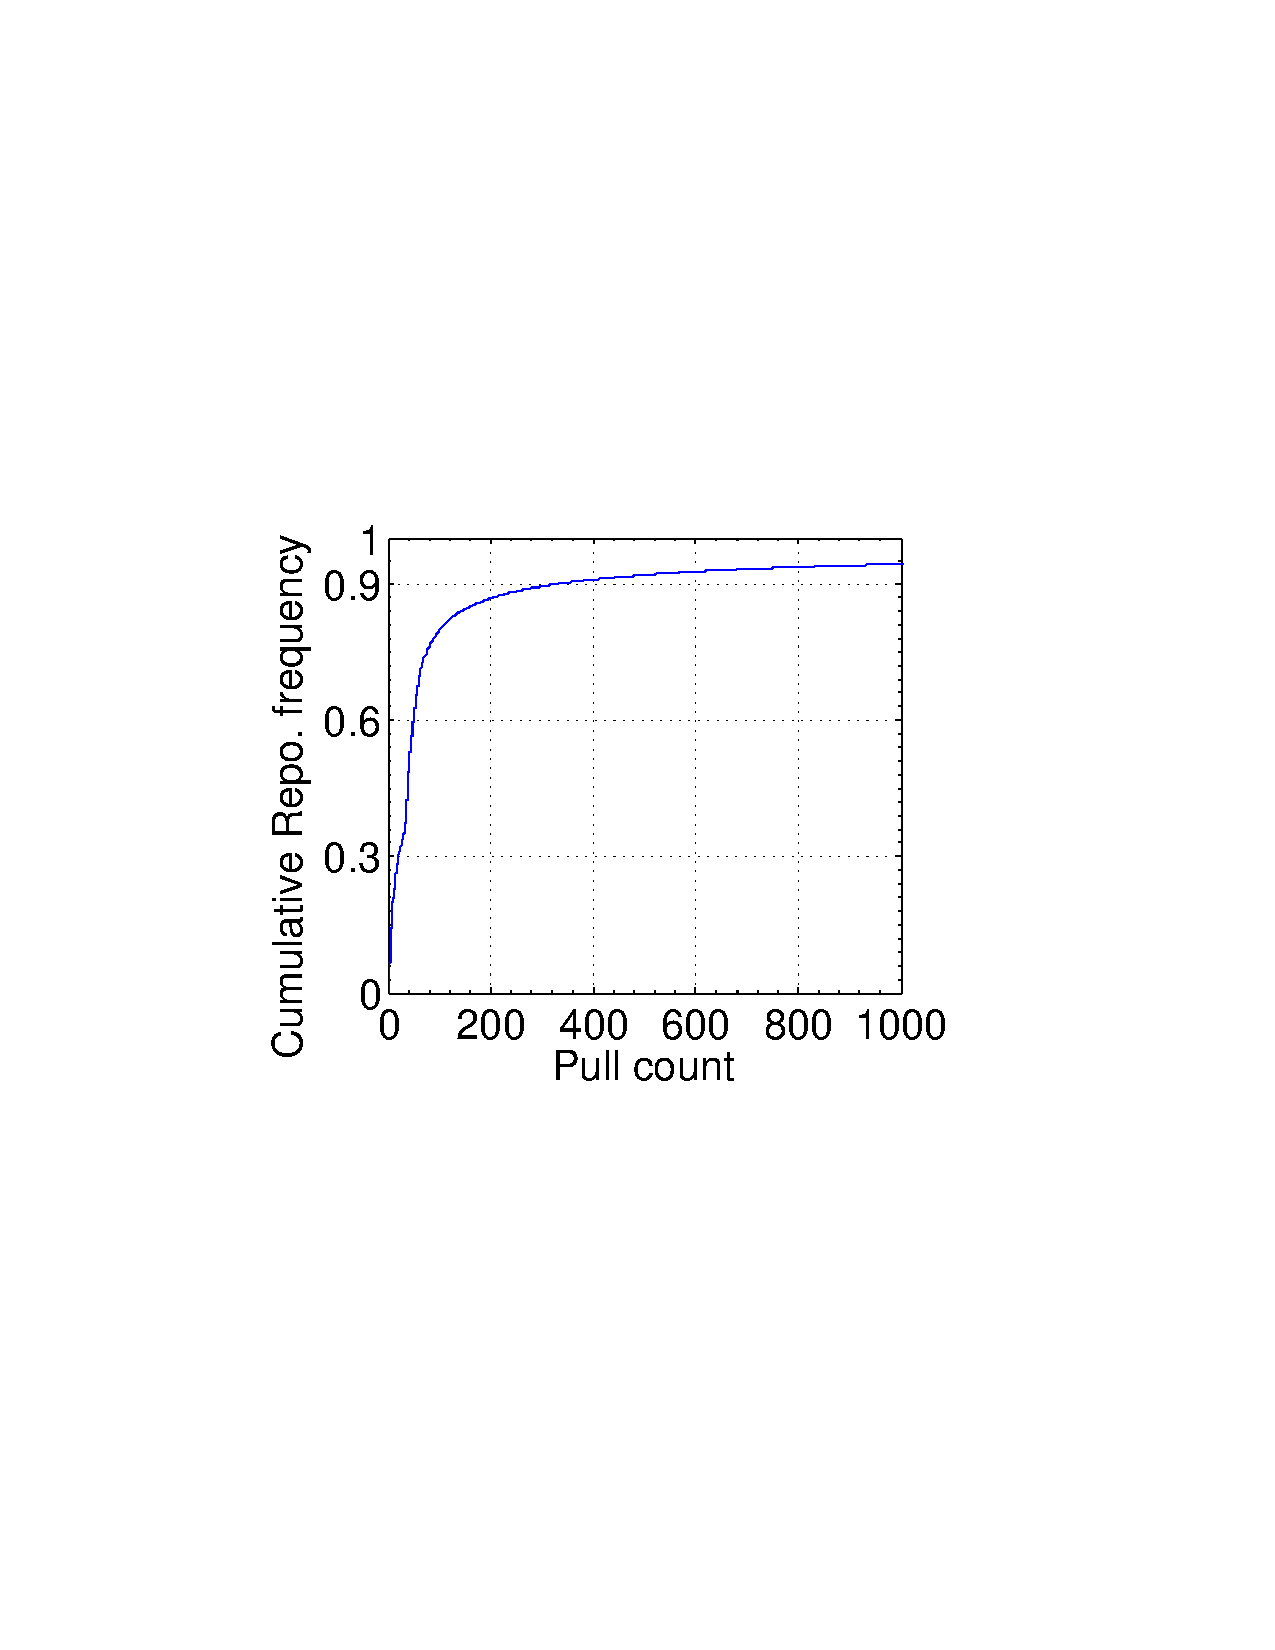
\includegraphics[width=0.23\textwidth]{graphs/pull_cnt.pdf}%
%	}
%	\subfigure[Histogram of repositories by pull count]{\label{fig_pull_cnt_count}
%		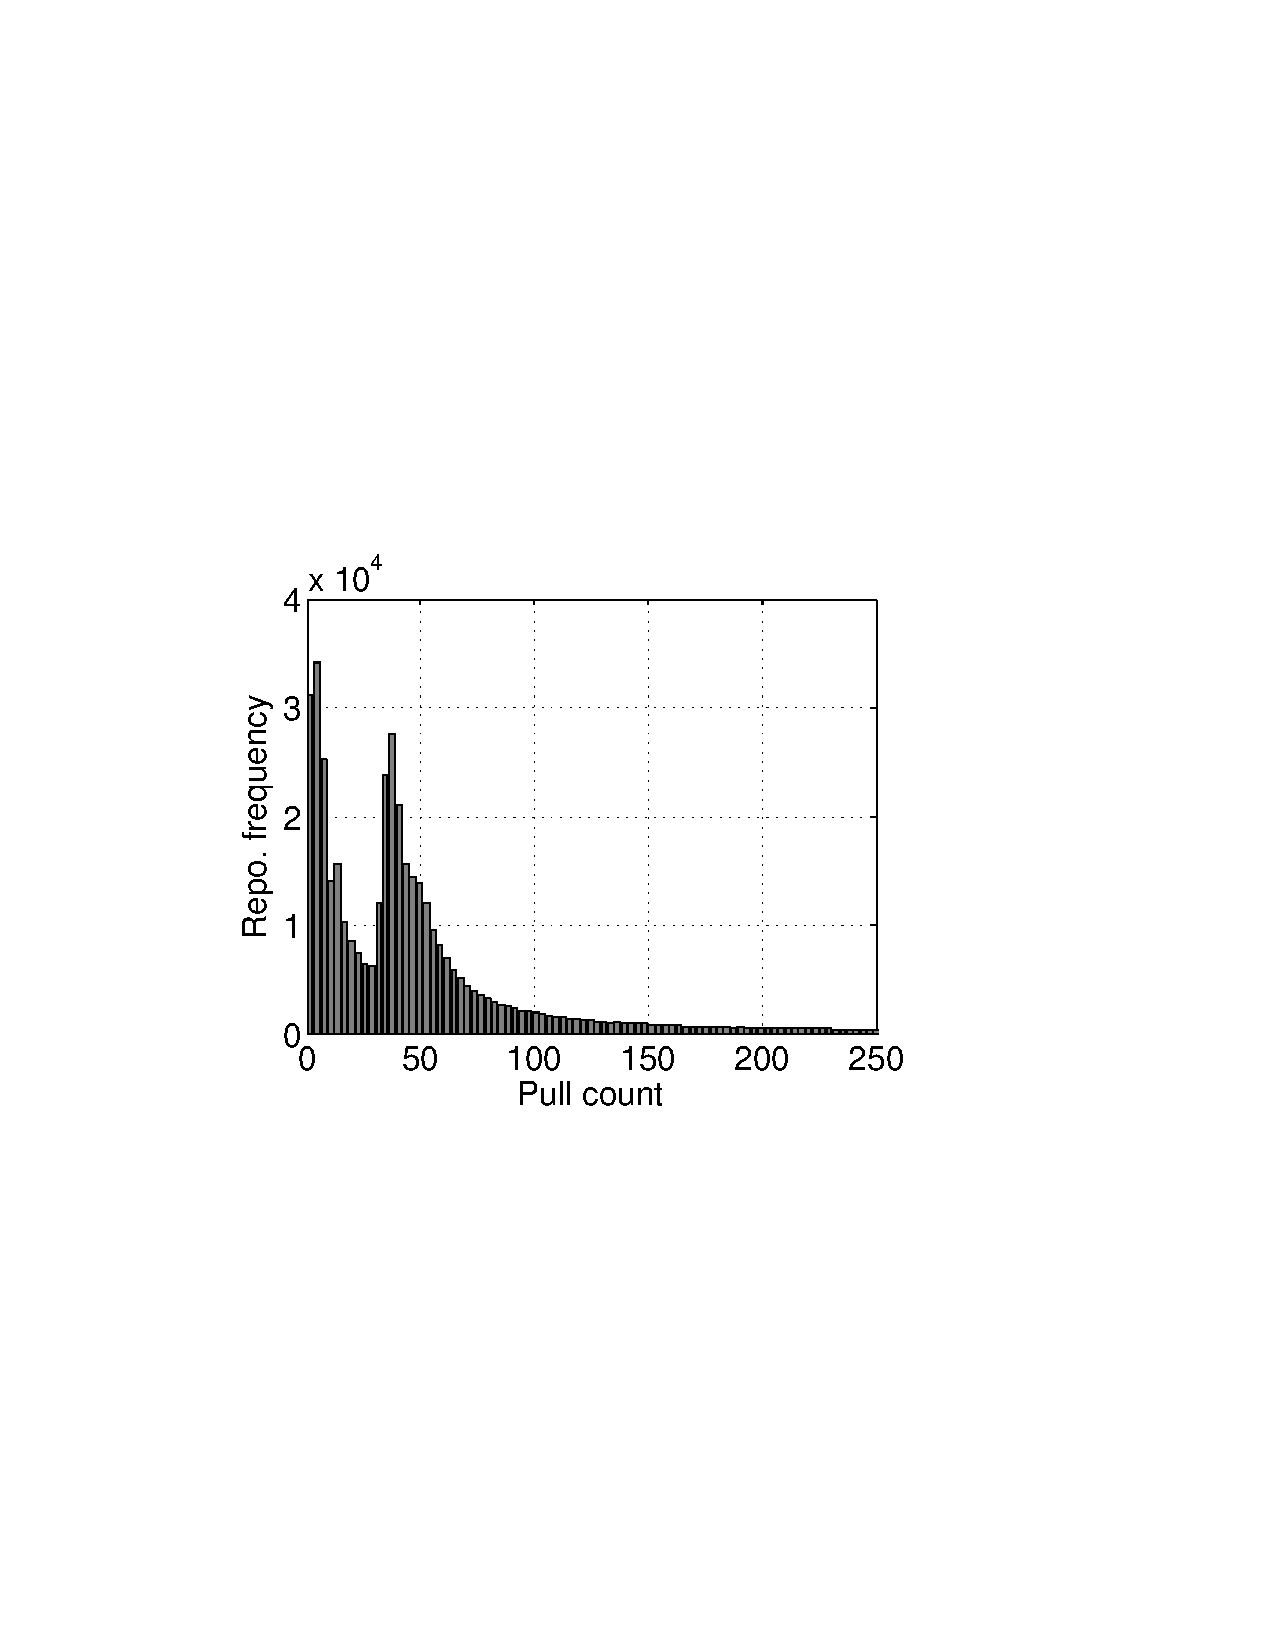
\includegraphics[width=0.22\textwidth]{graphs/count_pull_cnt.pdf}
%	}
%	\caption{Repository popularity distribution}
%	\label{fig-pop}
%\end{figure}

%=======================================
%|             OLD VERSION              |
%=======================================

%\paragraph{Latency distribution for each operation}
%\subsubsection{When to start file-level dedup?} 

%\paragraph{Latency distribution for each operation}

%\paragraph{Small compression ratio and small layer size}
%
%\begin{figure}[!t]
	\centering
	\subfigure[CDF of compression ratio]{\label{fig_cdf_compression_ratio}
		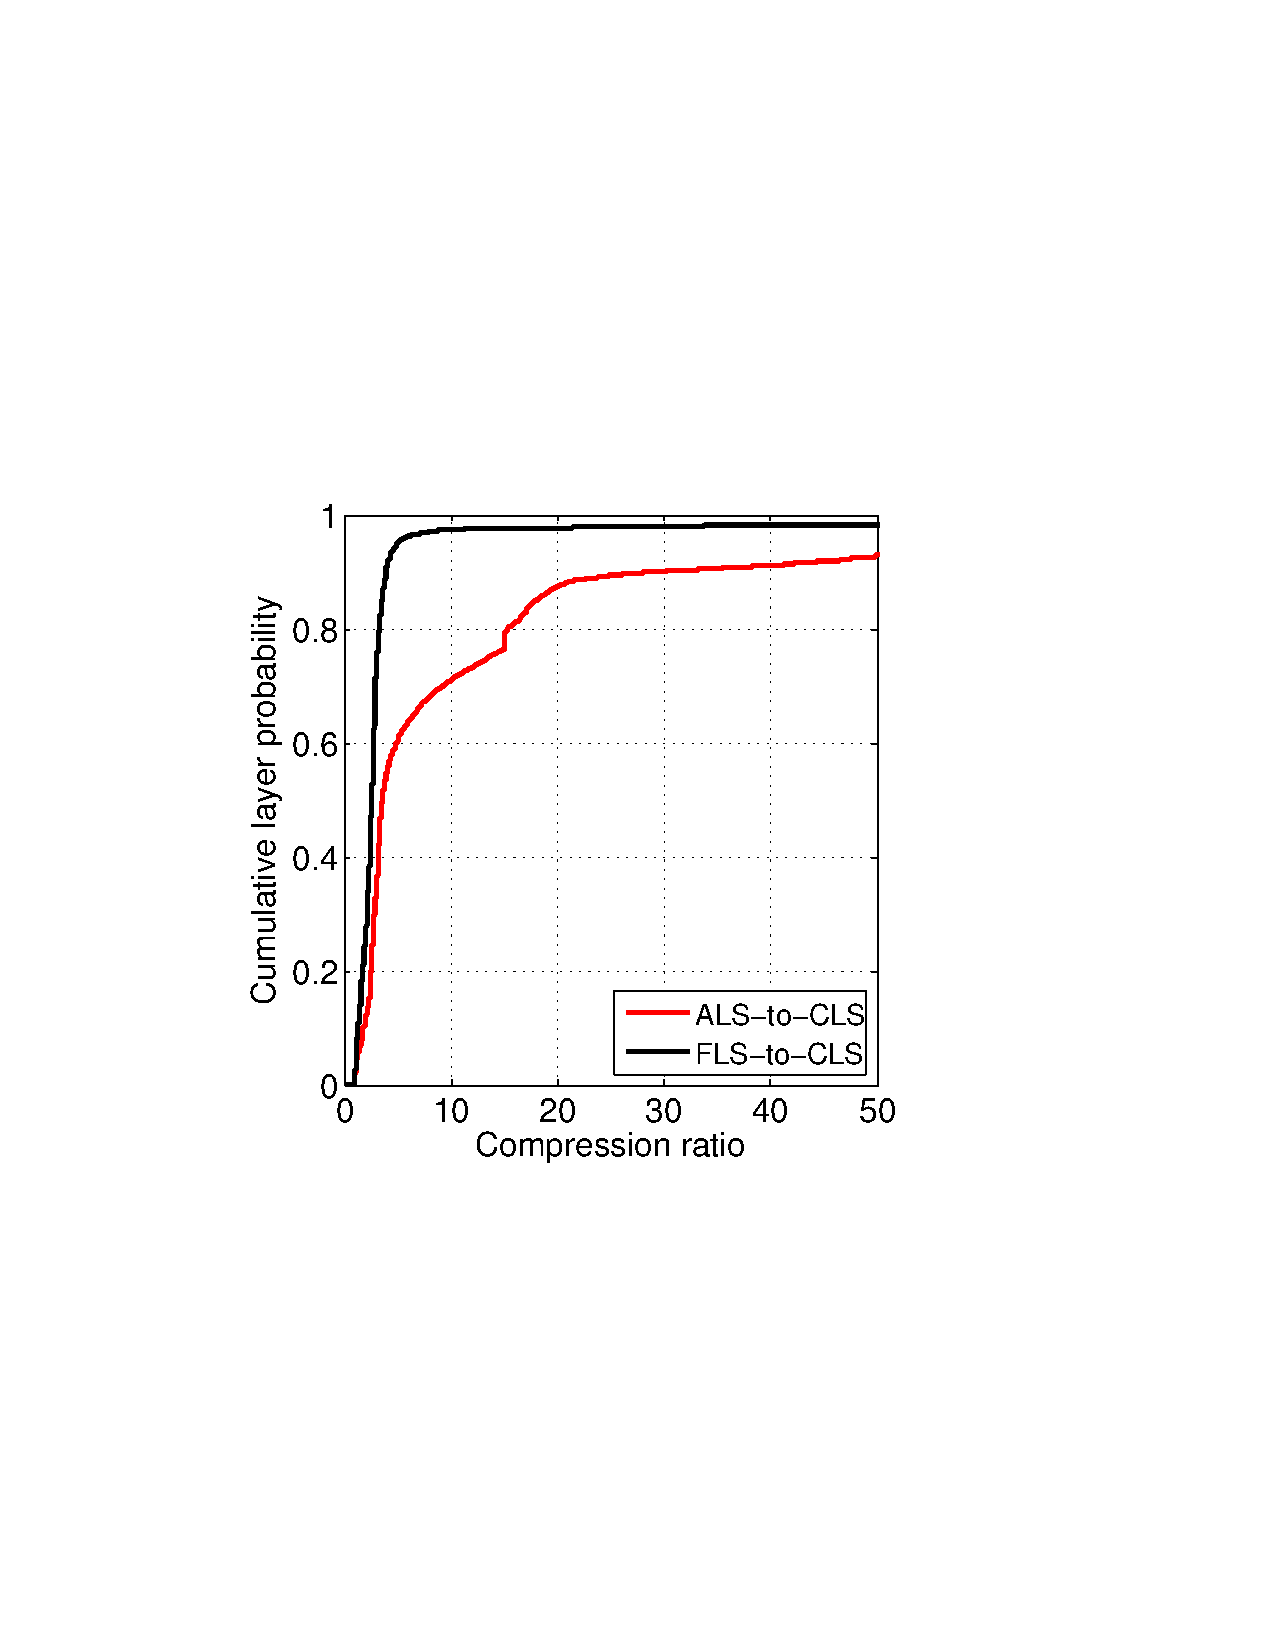
\includegraphics[width=0.23\textwidth]{graphs/cdf_compression_ratio.pdf}
	}
	\subfigure[Histogram of comp. ratios]{\label{fig_his_compression_ratio}
		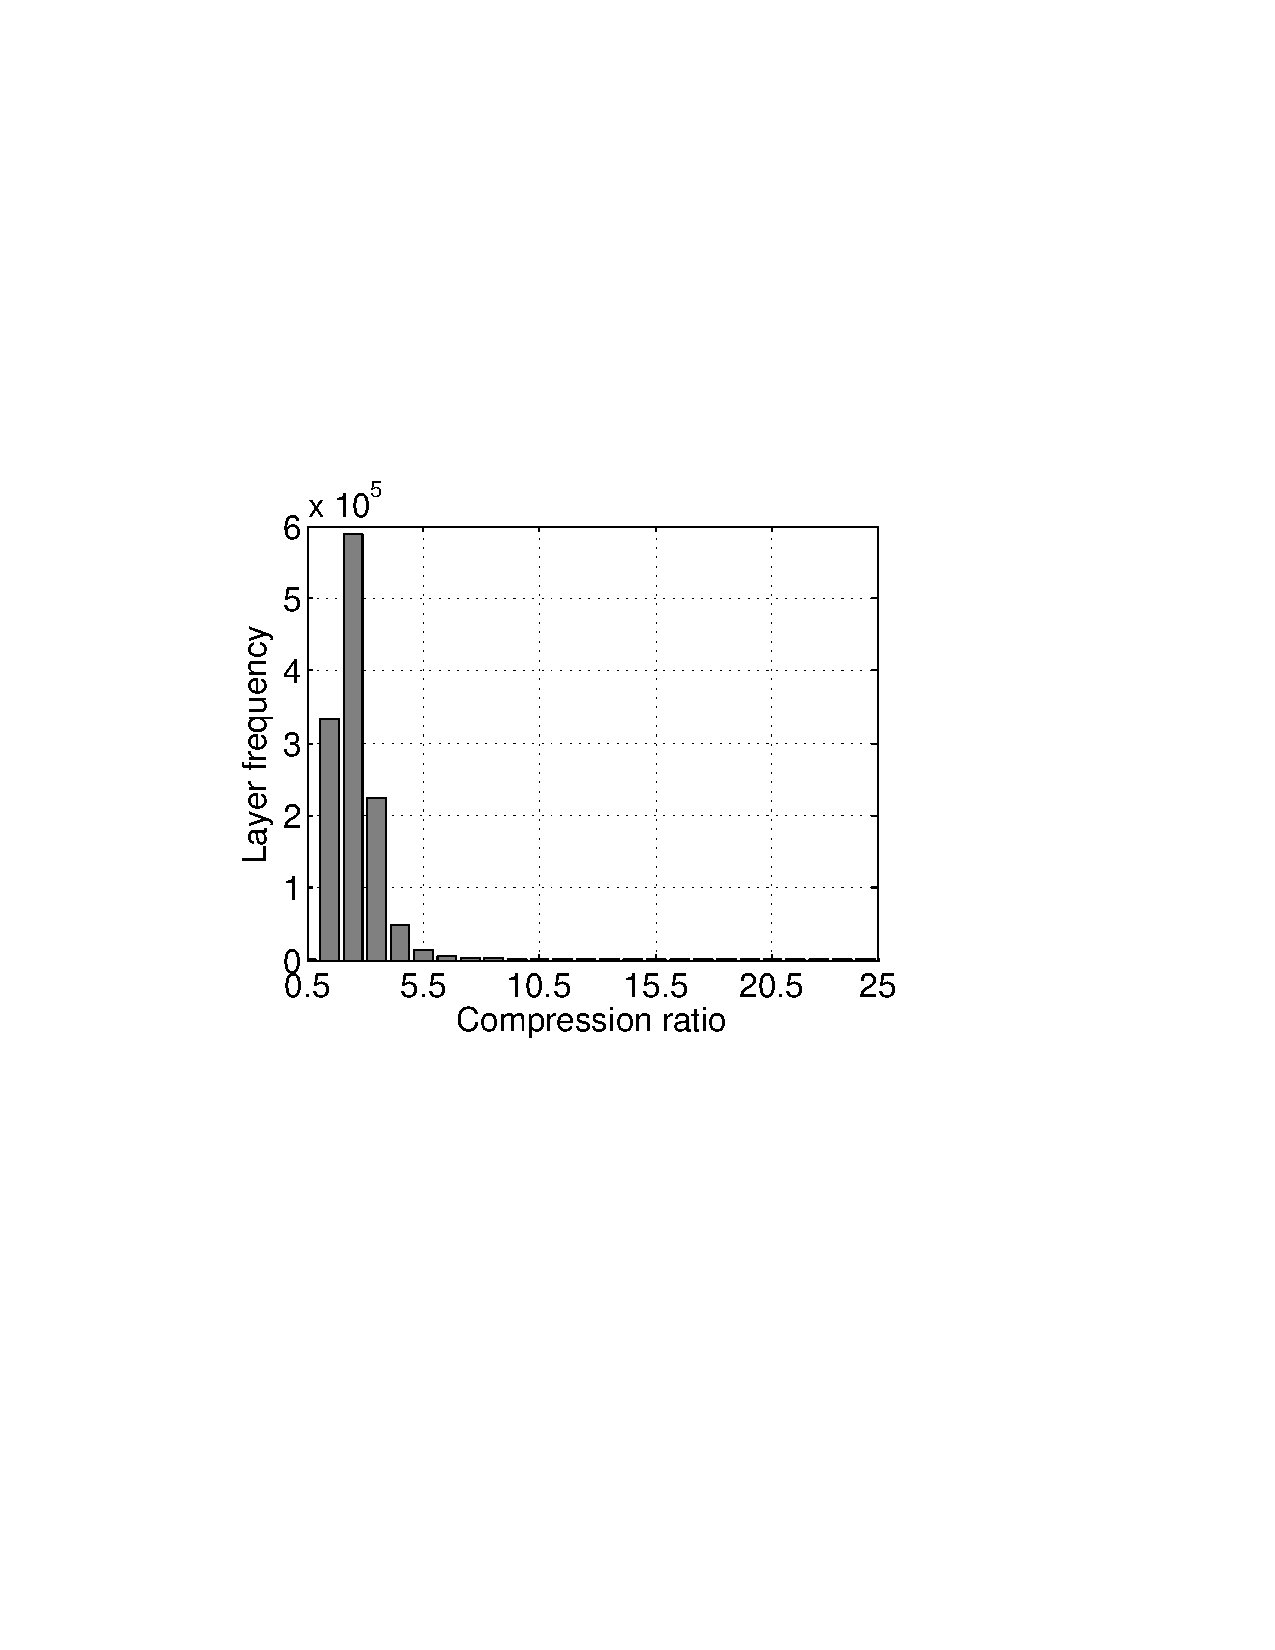
\includegraphics[width=0.223\textwidth]{graphs/his_compression_ratio.pdf}
	}
	\caption{Layer compression ratio distribution
	%\vcomment{Different colors are used in figure (a) and (b) FLS/CLS\nancomment{will address later}}
	}
	\label{fig-compression-ratio}
\end{figure}

%
%\begin{figure}[!t]
	\centering
	\subfigure[CDF of layer sizes]{\label{fig_layer_size_cdf}
		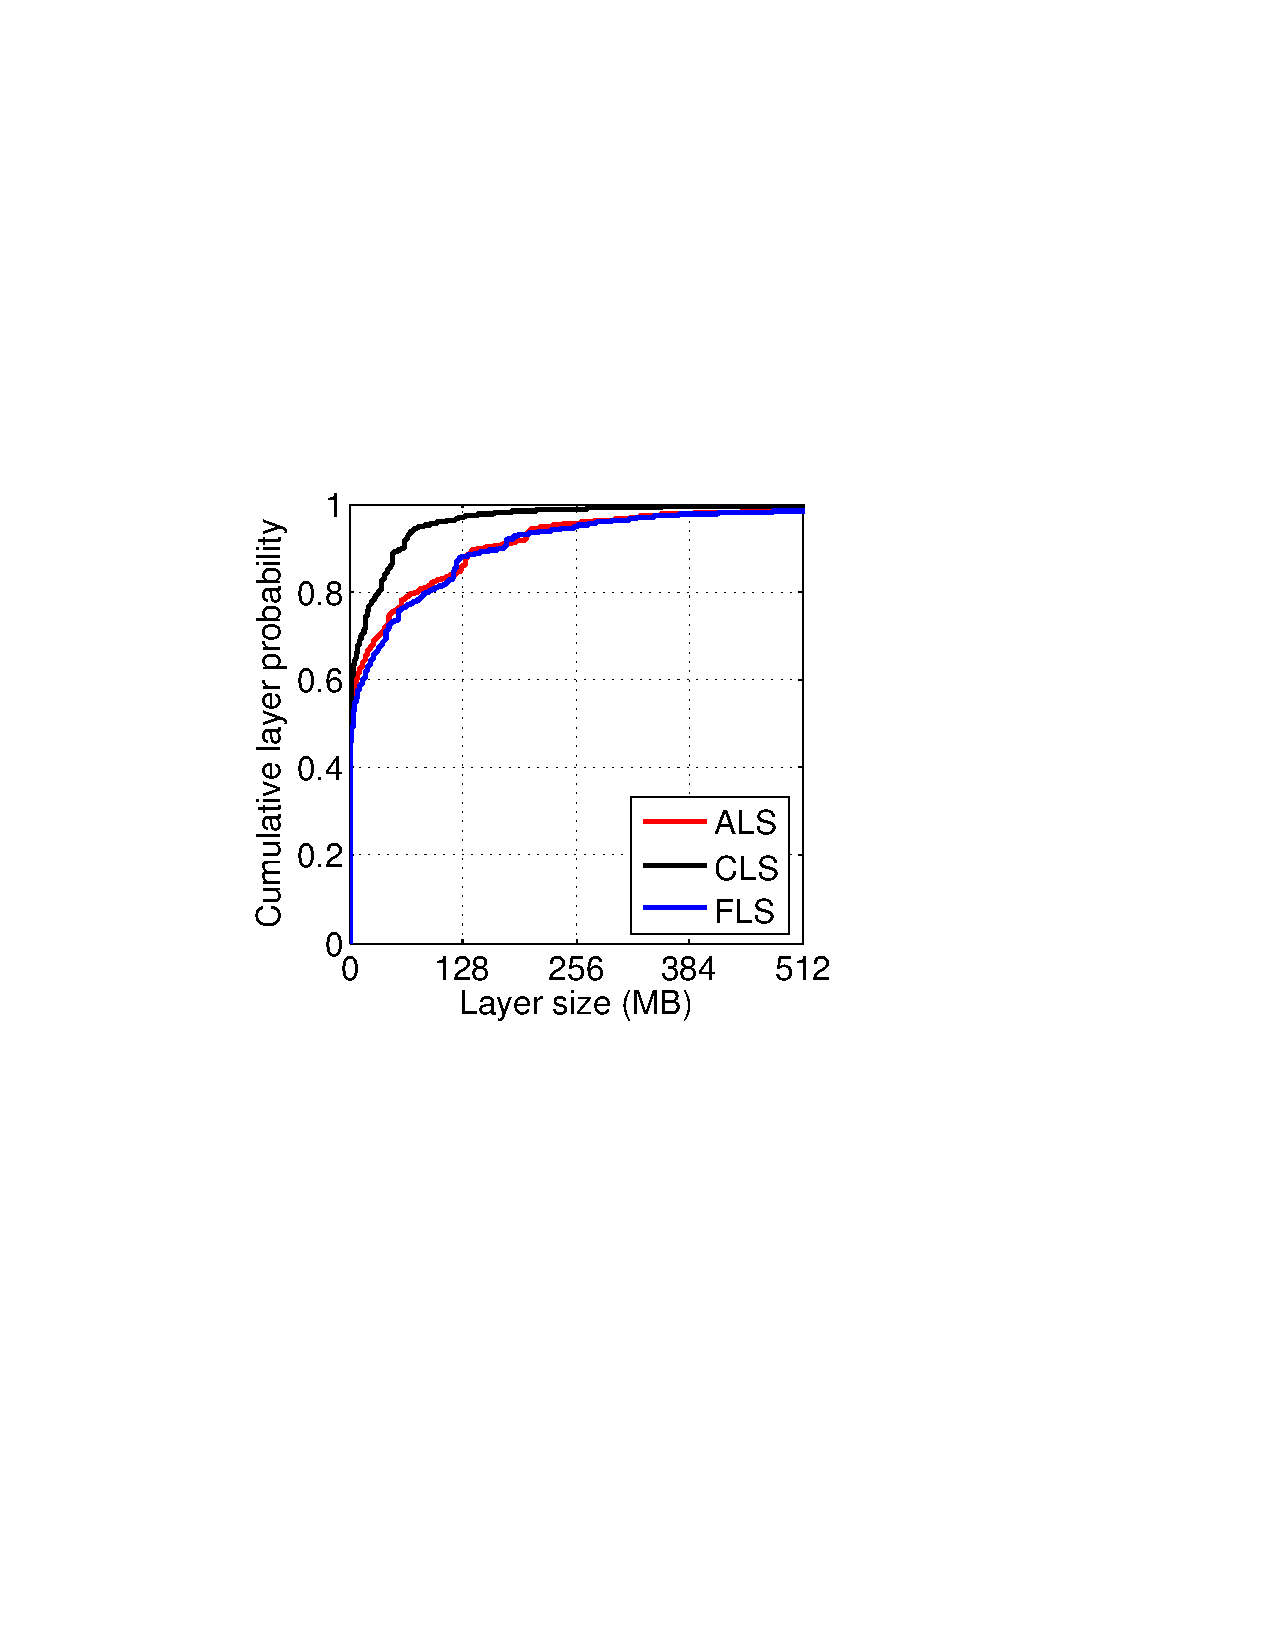
\includegraphics[width=0.234\textwidth]{graphs/layer_size_mb.pdf}
	}
	\subfigure[Histogram of layer sizes]{\label{fig_hist_layer_size}
		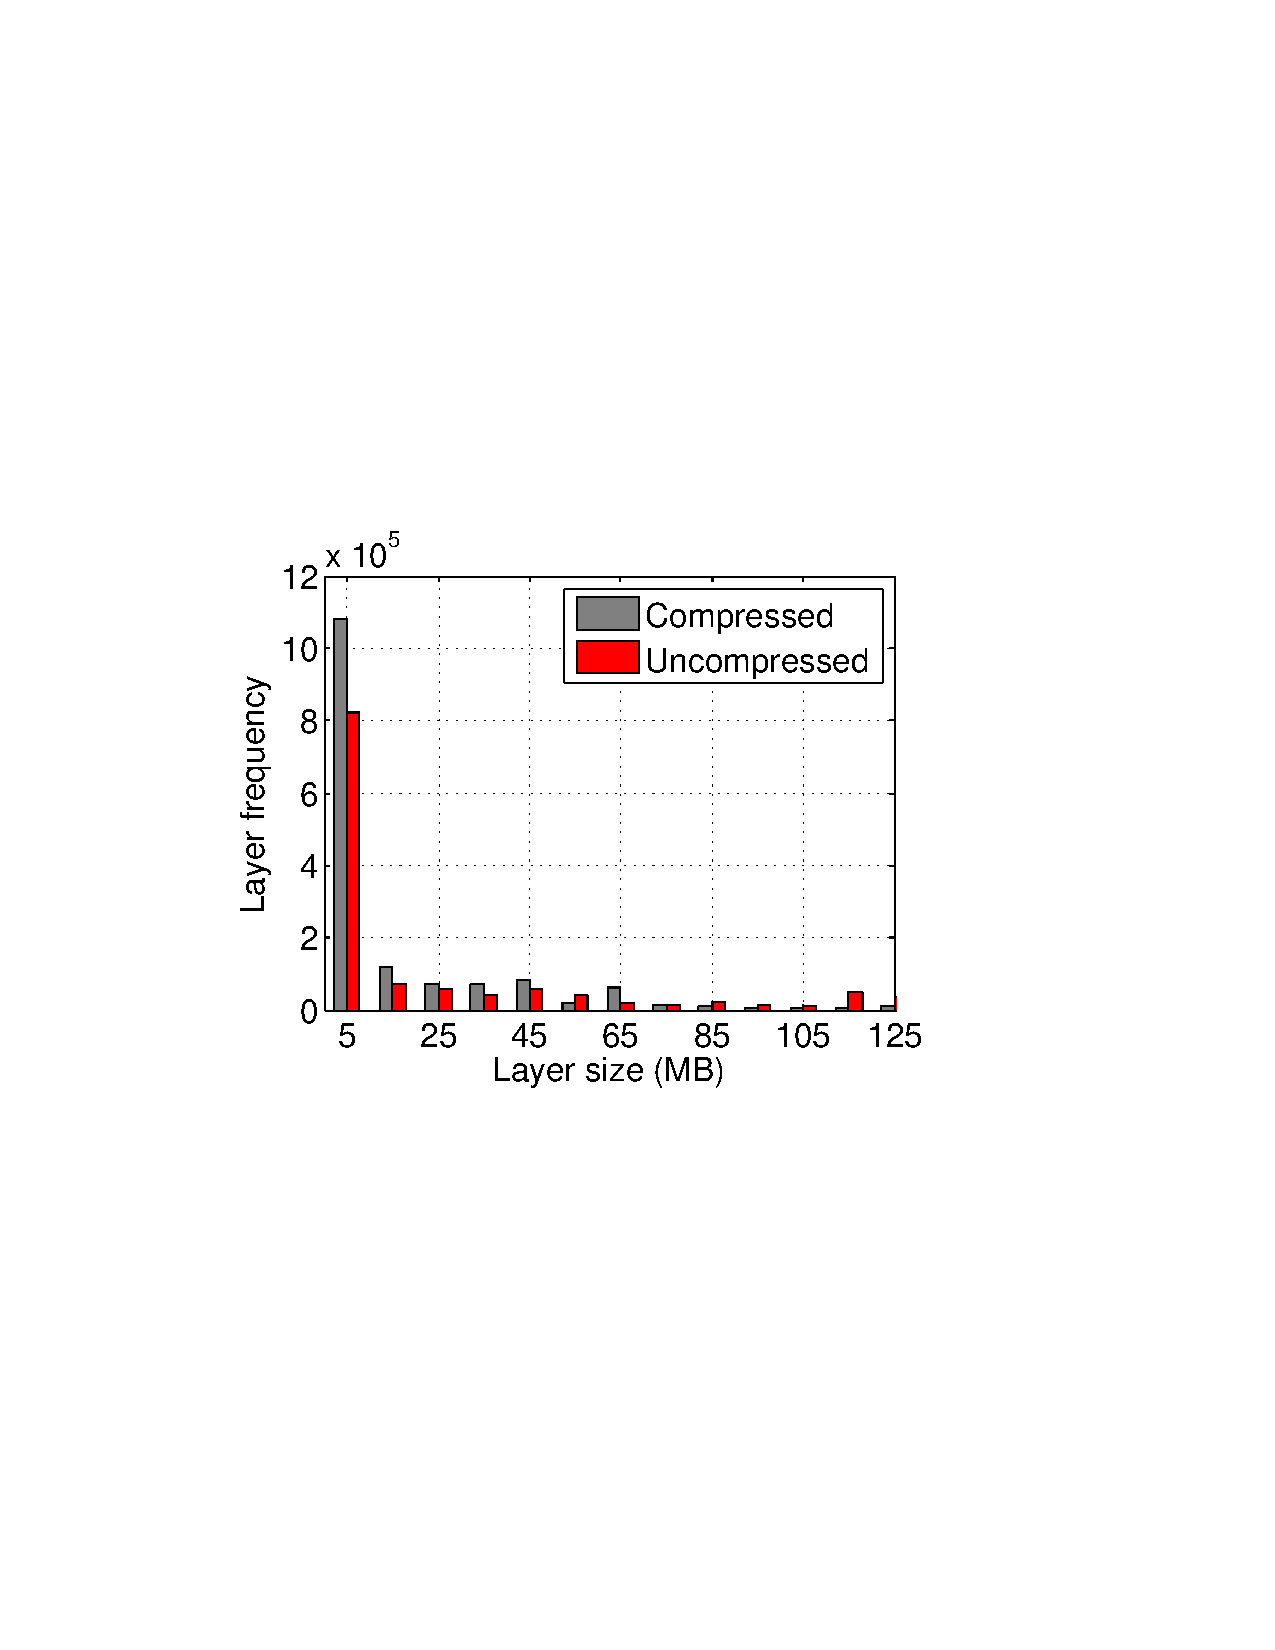
\includegraphics[width=0.213\textwidth]{graphs/hist_layer_size.pdf}
	}
	\caption{Layer size distribution
	\vcomment{Let's use CLS, ALS, and FLS abreviations\nancomment{addressed}}.
	\vcomment{CLS size should go first}.
	\vcomment{We need to use different types of lines (solid, dotted, etc.)
		or markers (round, triangular)}.
	\vcomment{In figure B it is not clear to which bar group corresponds
		  to which layer size. I suggest to try to rotate the graph
		  by 90 grads to fit all layer size labels.\nancomment{aligned label with bar}}
	}
	\label{fig-layer-size}
\end{figure}

%
%We found that most layers'compression ratio is really lower (?) while most of layers have a smaller size. 
%So how about we use archiving instead of compression if the network speed is higher (?GB/s)?

%\paragraph{Network transfer speed is high!}

%\subsubsection{File-level content addressable storage for cold layers}

%\begin{figure}
%	\centering
%	\includegraphics [width=0.45\textwidth]{plots/exp-total-stev-erase.eps}
%	\subfigure[]{\label{fig:per_layer_ratio_fcnt_cdf}
%		\includegraphics [width=0.23\textwidth]{graphs/}
%	}
%	\subfigure[Similar layer dedup]{\label{fig:per_layer_ratio_fcnt_pdf}
%		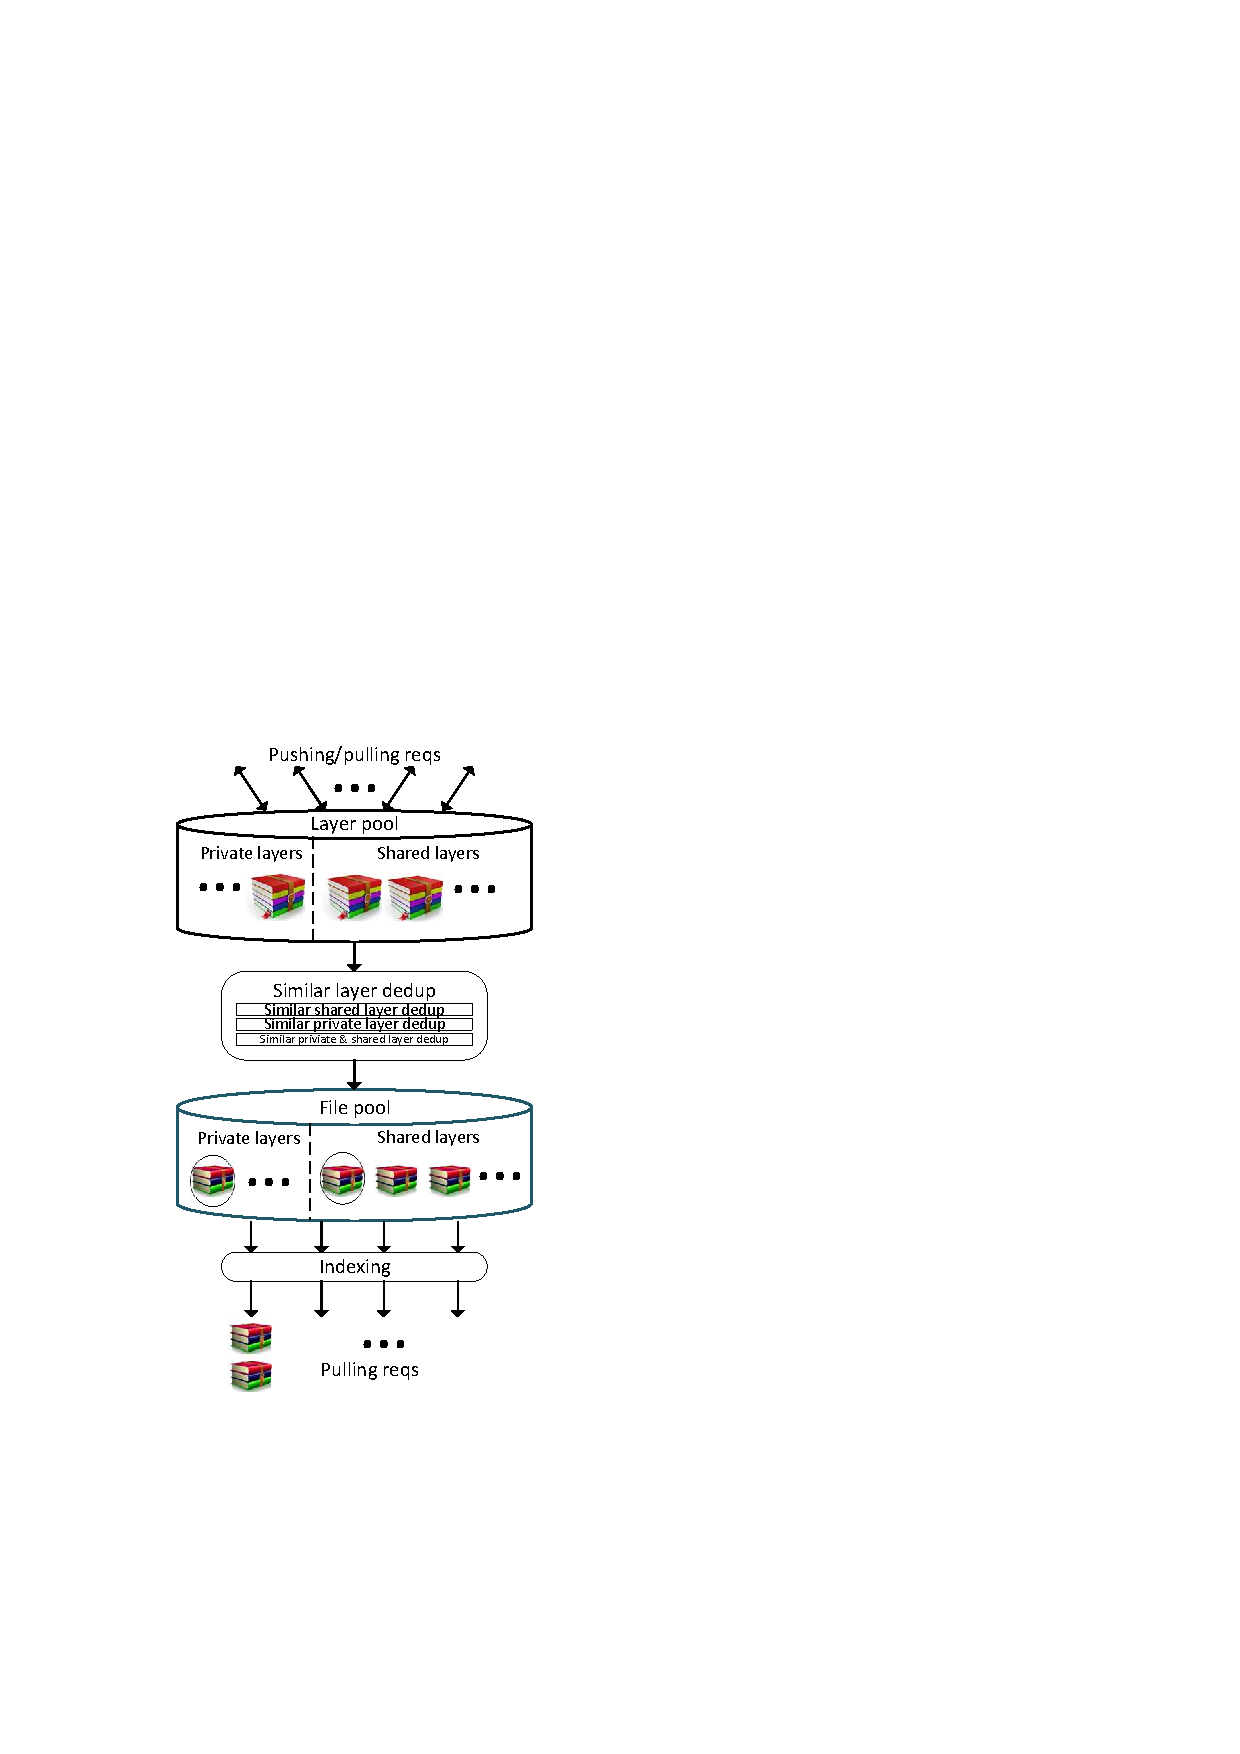
\includegraphics [width=0.22\textwidth]{graphs/graph_reconstruct_layers.pdf}
%	}
%	\caption{File-level content addressable storage model}
%	\label{fig:eval-stdev-erasure-cnt}
%\end{figure}

%\subsection{Hints for performance improvement and storage saving}

%\begin{table} 
%	\centering 
%	\scriptsize  
%	%\begin{minipage}{.5\linewidth}
%	\caption{Latency breakdown} \label{tbl:latency_breakdown} 
%	\begin{tabular}{|l|l|l|l|l|}%p{0.14\textwidth} 
%		\hline 
%		% after \\: \hline or \cline{col1-col2} \cline{col3-col4} ... 
%		% after \\: \hline or \cline{col1-col2} \cline{col3-col4} ... 
%		Operations/latency (S) & max & min & median & avg.\\
%		\hline
%		 gunzip decompression (RAM) & 257.16  & 0.04  & 0.15  & 0.39 \\
% 		\hline
% 		tar extraction (RAM) & 43.41  & 0.04  &  0.14  & 0.18 \\
%		\hline
%		Digest calculation (RAM) & 3455.01  & $<$0.00  & 0.05 & 10.65 \\
%		\hline
%		tar archiving (RAM)  & 53.44 & 0.04 & 0.14 & 0.19\\
%		\hline
%		gzip compression (RAM) & 496.04 & 0.04 & 0.15 & 2.10 \\
%%		\hline
%%		Total time (RAM) (with compression) & & & & \\
%%		\hline
%%		Total time (RAM) (without compression) & & & & \\
%		\hline
% 		\hline
% 		gunzip decompression (SSD) &   &   &    &  \\
% 		\hline
% 		tar extraction (SSD) &   &   &    &  \\
%		\hline
%		Digest calculation (SSD) &  &  & & \\
%		\hline
%		tar archiving (SSD) &  &  & & \\
%		\hline
%		gzip compression (SSD) & &  &  & \\
%%		\hline		 
%%		Total time (SSD) (with compression) & & & & \\
%%		\hline
%%		Total time (SSD) (without compression) & & & & \\
%		\hline
%		\hline
%		Network transfer & 20587.94 & $<$ 0.00 & $<$ 0.00 & 1.20 \\
%		\hline 	
%	\end{tabular} 
%\end{table}


%\begin{table} 
%	\centering 
%	\scriptsize  
%	%\begin{minipage}{.5\linewidth}
%	\caption{Summary of layer \& image characterization} \label{tbl:redundant_ratio} 
%	\begin{tabular}{|l|l|l|l|l|}%p{0.14\textwidth} 
%		\hline 
%		% after \\: \hline or \cline{col1-col2} \cline{col3-col4} ... 
%		% after \\: \hline or \cline{col1-col2} \cline{col3-col4} ... 
%		Metrics & max & min & median & avg.\\
%		\hline
%		Compressed layer size &   &   &   &  \\
%		\hline
%		Uncompressed layer size &   &   &    &  \\
%		\hline
%		Archival size &  &  & & \\
%		\hline
%		Compression ratio &   &   &    &  \\
%		\hline
%		Layer pull cnt. &  &  & & \\
%		\hline
%		File cnt. per layer &  &  & & \\
%		\hline
%		Dir. cnt. per layer &  &  & & \\
%		\hline
%		Layer depth &  &  & & \\
%		\hline
%		\hline
%		Compressed image size &  &  & & \\
%		\hline
%		Uncompressed image size & &  &  & \\
%		\hline
%		Archival image size & &  &  & \\
%		\hline
%		Compression ratio &   &   &    &  \\
%		\hline
%		Image pull cnt.  &  &  & & \\
%		\hline
%		Layer cnt. per image  &  &  & & \\
%		\hline
%		Shared layer cnt. per image  &  &  & & \\
%		\hline
%		File cnt. per layer &  &  & & \\
%		\hline
%		Dir. cnt. per layer &  &  & & \\
%		\hline	
%	\end{tabular} 
%\end{table} 

%\subsection{Constructing shared layers for redundant directories/files}
%
%\paragraph{Smaller number of layers are shared among different images}
%\begin{figure}[!t]
	\centering
	\subfigure[CDF of layer reference count]{\label{fig_repeate_layer}
		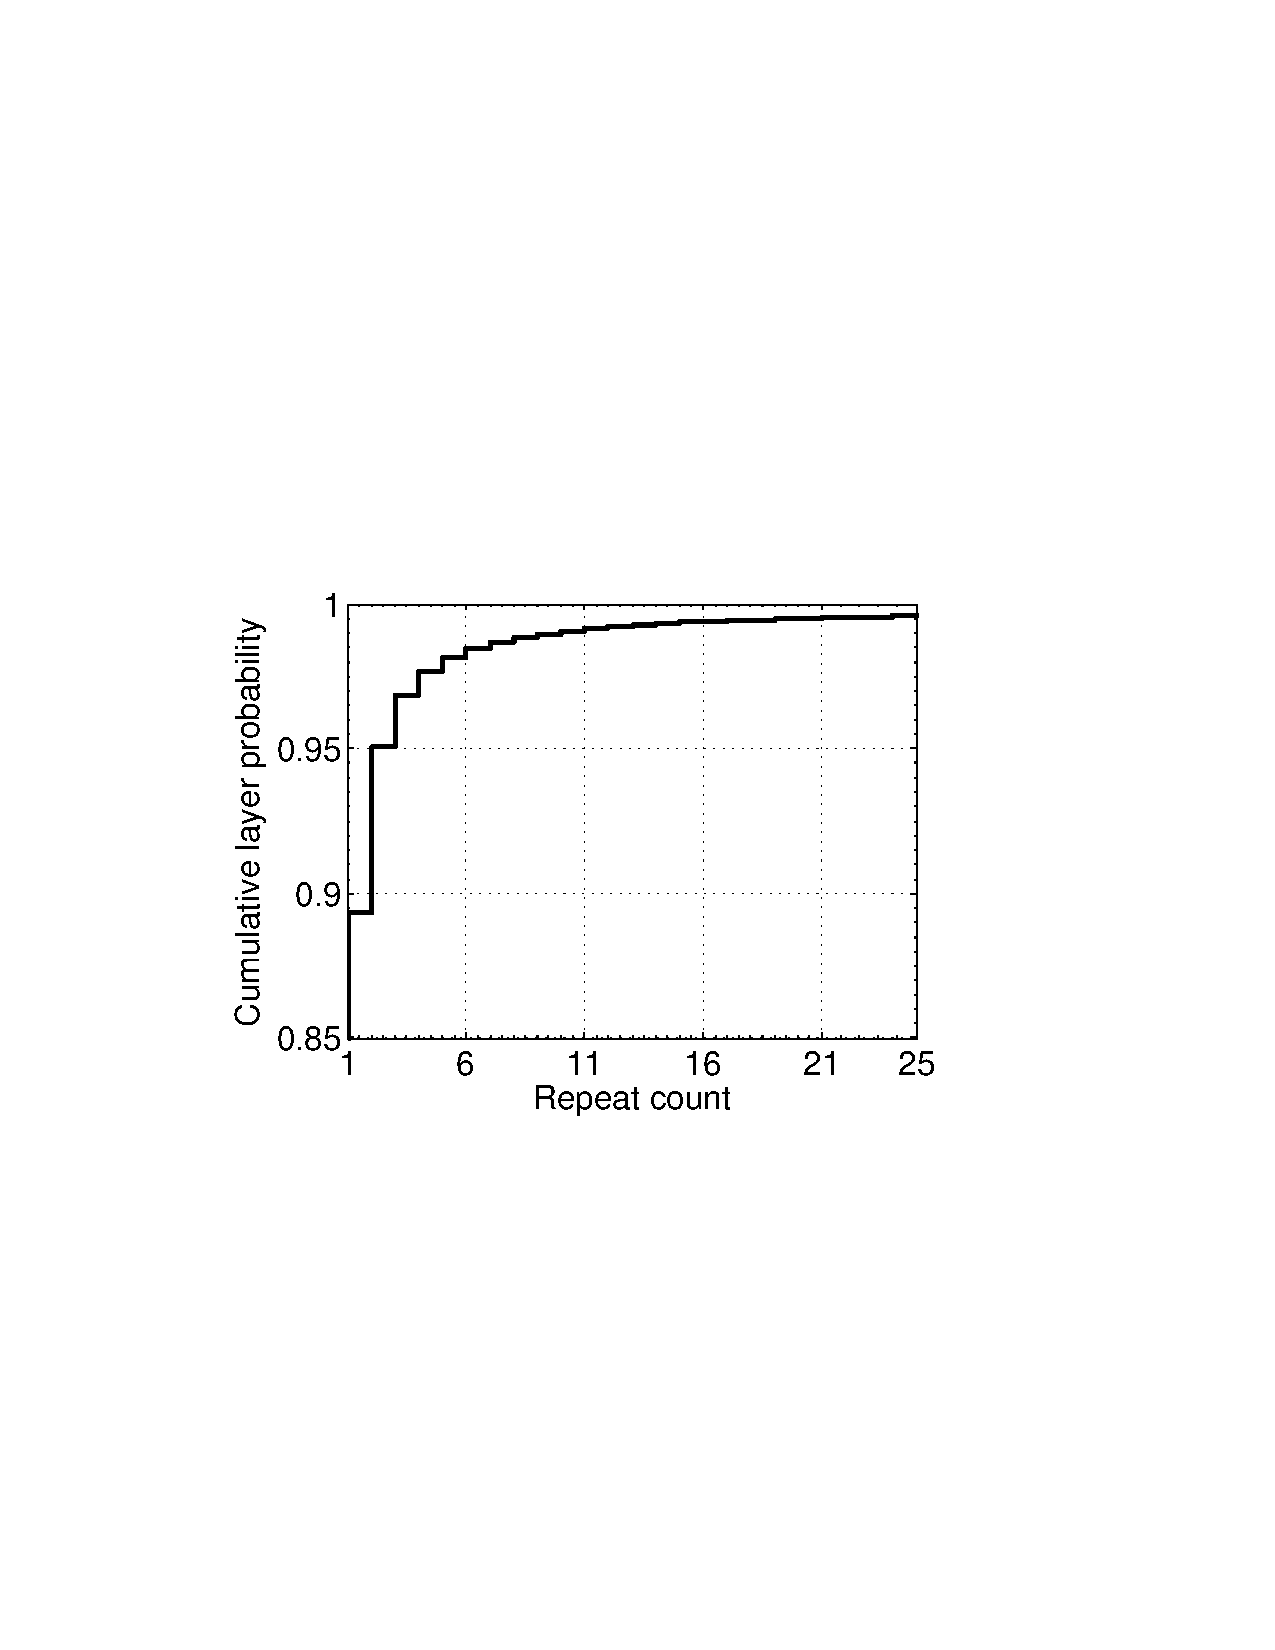
\includegraphics[width=0.23\textwidth]{graphs/repeate_layer.pdf}
	}
	\subfigure[Histogram of layer reference count]{\label{fig_hist_repeate_layer}
		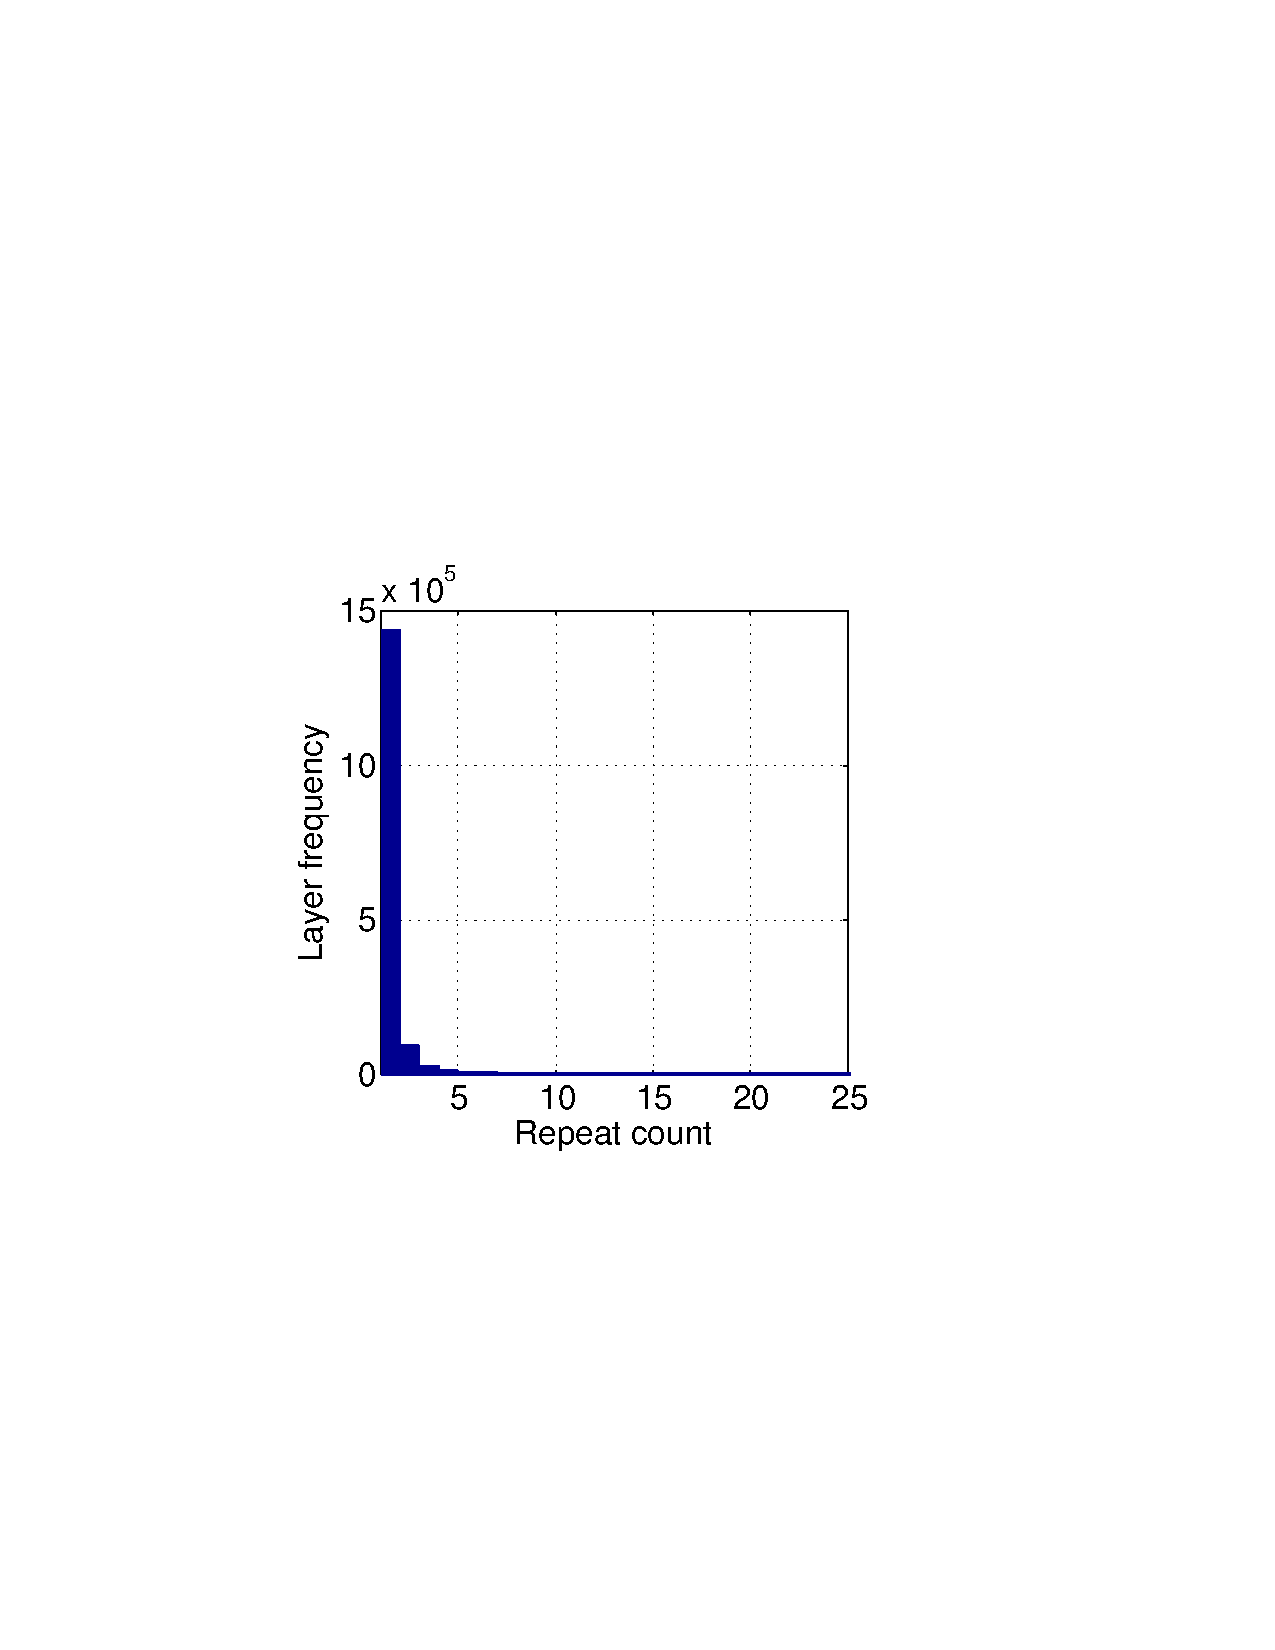
\includegraphics[width=0.223\textwidth]{graphs/hist_repeate_layer.pdf}
	}
	\caption{Layer reference counts across all images}
	\label{fig-repeat-layer-cnt}
\end{figure}
%
%\paragraph{Smaller pull latency than recompression model} the registry can prepare the reconstructed layers before users issue a pull request. But this model requires users to rebuild two layers.

%\subsubsection{Summary of Suggestions/trade-offs between dedup ratio and recompression overhead}
%
%\paragraph{1. using archiving instead of compression}
%\paragraph{2. using file-level dedup for cold images/layers}
%\paragraph{3. using file-level dedup economically}
%When to trigger file-level dedup?
%\paragraph{4. constructing shared layers for redundant dirs/files, for example,}
%%\subsection{Layer reconstruction model}
%%\subsubsection{Reconstruction overhead}
%%\subsubsection{Trade-offs between dedup ratio and reconstruction overhead}
%%\paragraph{Dedup ratio VS. Rebuild overhead}
%%\subsection{Evaluation results}
